\newpage \ \thispagestyle{empty} \newpage
\chapter{Retrospettiva delle attività}
\label{cap:resoconto}
Questo capitolo contiene una valutazione retrospettiva sulle attività svolte ed il risultato ottenuto, mettendo a confronto:
\begin{itemize}
    \item Aspettive e risultati raggiunti;
    \item Competenze acquisite durante le attività e competenze erogate dal corso di studi.
\end{itemize}

\section{Raggiungimento degli obiettivi prefissati}
% In questa sezione metterò in relazione gli obiettivi indicati in §2.5 ed i risultati indicati in §3.8.

\subsection{Obiettivi aziendali}
Gli obiettivi che riporto di seguito fanno riferimento alla sezione \hyperref[sec:obiettivi-aziendali]{§2.3}.
\subsubsection*{Obiettivi obbligatori}
\rowcolors{2}{white}{gray!25}
\begin{longtable}{>{\centering\arraybackslash}m{0.50\textwidth}>{\centering\arraybackslash}m{0.15\textwidth}>{\centering\arraybackslash}m{0.35\textwidth}}
    \hline
    \rowcolor{black}
    \color{white}\textbf{Obiettivo} & \color{white}\textbf{Soddisfatto} & \color{white}\textbf{Fonte} \\
    \hline
    \endhead % This line indicates the end of the header and the start of the repeated heading on subsequent pages
    \textbf{O01}: comprensione dei requisiti utente da soddisfare & SÌ & \hyperref[sec:analisi]{§3.3} Analisi, \hyperref[sec:validazione]{§3.7} Validazione \\
    \hline
    \textbf{O02}: studio dell’interfaccia dell’applicazione \textit{ADeMES}, che verrà integrata con il prodotto da sviluppare durante il tirocinio & SÌ & Tabella \hyperref[tab:colors]{3.7} \\
    \hline
    \textbf{O03}: acquisizione della sufficiente dimestichezza con i concetti di base del \textit{framework Angular} & SÌ & \hyperref[subsec:architettura]{§3.4.3} Progettazione - Architettura \\
    \hline
    \textbf{O04}: progettazione dell'interfaccia grafica in base allo stile dell'interfaccia dell'applicazione \textit{ADeMES} & SÌ & \hyperref[subsec:interfaccia]{§3.4.2} Progettazione - Interfaccia grafica  \\
    \hline
    \textbf{O05}: sviluppo di una versione di base dell'applicazione \textit{web} che consenta di eseguire le operazioni \textit{CRUD} sui dati di qualità & SÌ & \hyperref[sec:validazione]{§3.7} Validazione \\
    \hline
    \textbf{O06}: \textit{live demo} della web application in un ambiente simulato & SÌ & \hyperref[sec:validazione]{§3.7} Validazione \\
    \hline
    \textbf{O07}: studio e scelta (motivata) della tecnologia per la fruizione dell'applicazione in lingua inglese & SÌ & \hyperref[subsec:internazionalizzazione]{§3.4.1} Internazionalizzazione e localizzazione \\
    \hline
    \textbf{O08}: il \textit{software} deve potersi integrare nel \textit{software} ADeMES mediante un elemento \texttt{<iframe>} \textit{HTML} & SÌ & \hyperref[subsec:integrazione]{§3.5} Codifica - Integrazione dell'applicazione con \textit{ADeMES}\\
    \hline
    \textbf{O09}: il \textit{software} deve poter essere eseguibile in modalità \textit{standalone} (in questo caso, in grado di funzionare anche senza l'ausilio del \textit{software ADeMES}) & SÌ & \hyperref[subsec:interfaccia-risultato]{§3.8.2} Risultato finale - interfaccia grafica \\
    \hline
    \caption{Obiettivi di tirocinio - obbligatori}
\end{longtable}

\subsubsection*{Obiettivi desiderabili}
\rowcolors{2}{white}{gray!25}
\begin{longtable}{>{\centering\arraybackslash}m{0.50\textwidth}>{\centering\arraybackslash}m{0.15\textwidth}>{\centering\arraybackslash}m{0.35\textwidth}}
    \hline
    \rowcolor{black}
    \color{white}\textbf{Obiettivo} & \color{white}\textbf{Soddisfatto} & \color{white}\textbf{Fonte} \\
    \hline
    \endhead % This line indicates the end of the header and the start of the repeated heading on subsequent pages
    \textbf{D01}: ottimizzazione dei servizi esposti & NO & - \\
    \hline
    \caption{Obiettivi di tirocinio - desiderabili}
\end{longtable}
L'obiettivo \textbf{D01} non è stato soddisfatto a causa del poco tempo rimanente al termine delle attività di sviluppo del \textit{software ADeQA}.

\subsubsection*{Obiettivi facoltativi}
\rowcolors{2}{white}{gray!25}
\begin{longtable}{>{\centering\arraybackslash}m{0.50\textwidth}>{\centering\arraybackslash}m{0.15\textwidth}>{\centering\arraybackslash}m{0.35\textwidth}}
    \hline
    \rowcolor{black}
    \color{white}\textbf{Obiettivo} & \color{white}\textbf{Soddisfatto} & \color{white}\textbf{Fonte} \\
    \hline
    \endhead % This line indicates the end of the header and the start of the repeated heading on subsequent pages
    \textbf{F01}: ottimizzazione dell'esperienza utente per compatibilità con \textit{ADeMES} & SÌ & \hyperref[sec:validazione]{§3.7} Validazione \\
    \hline
    \textbf{F02}: ottimizzazione dell'interfaccia grafica, per rendere quanto più simile il prodotto a \textit{ADeMES} & SÌ & Tabella \hyperref[tab:colors]{3.7} \\
    \hline
    \textbf{F03}: possibilità di fruizione dell'applicazione in lingua spagnola & SÌ & \hyperref[subsec:internazionalizzazione]{§3.4.1} Internazionalizzazione e localizzazione \\
    \hline
    \caption{Obiettivi di tirocinio - facoltativi}
\end{longtable}

\subsection{Obiettivi personali}
Gli obiettivi che riporto di seguito fanno riferimento alla sezione \hyperref[sec:obiettivi-personali]{§2.6}.

\rowcolors{2}{white}{gray!25}
\begin{longtable}{>{\centering\arraybackslash}m{0.50\textwidth}>{\centering\arraybackslash}m{0.15\textwidth}>{\centering\arraybackslash}m{0.35\textwidth}}
    \hline
    \rowcolor{black}
    \color{white}\textbf{Obiettivo} & \color{white}\textbf{Soddisfatto} & \color{white}\textbf{Fonte} \\
    \hline
    \endhead % This line indicates the end of the header and the start of the repeated heading on subsequent pages
    Capire come convertire una \textit{web application} in una \textit{Progressive Web App} & SÌ & \hyperref[sec:validazione]{§3.7} Validazione \\
    \hline
    Sviluppare un'interfaccia grafica che si adatti a \textit{desktop}, \textit{tablet} e \textit{smartphone} & SÌ & \hyperref[subsec:interfaccia]{§3.4.2} Progettazione - Interfaccia grafica \\
    \hline
    Comprendere come rendere fruibile in più lingue un prodotto \textit{software} & SÌ & \hyperref[subsec:internazionalizzazione]{§3.4.1} Internazionalizzazione e localizzazione \\
    \hline
    Capire come si possono gestire diversi temi grafici (tipicamente identificati come "tema chiaro" e "tema scuro") in un'interfaccia grafica \textit{web} \textit{software} & SÌ & \hyperref[subsec:interfaccia-risultato]{§3.8.2} Risultato finale - interfaccia grafica \\
    \hline
    Ideare un prodotto in grado di integrarsi con successo in un \textit{software} già esistente & SÌ & \hyperref[sec:validazione]{§3.7} Validazione \\
    \hline
    \caption{Obiettivi di tirocinio - personali}
\end{longtable}

\subsection{Commento}
Ho conseguito in modo soddisfacente quasi tutti gli obiettivi nel corso delle attività di tirocinio, in particolare tutti gli obiettivi obbligatori aziendali e gli obiettivi personali: valuto positivamente l'esperienza di \textit{stage} sia per quanto concerne il risultato raggiunto, 
sia per le modalità ed il clima di svolgimento delle attività.

\section{Competenze e conoscenze acquisite}
% In questa sezione descriverò le abilità e le conoscenze acquisite nel corso del tirocinio indicando (se necessario) i benefici ottenuti ed il loro grado di acquisizione.
Durante le attività di tirocinio ho potuto affinare e acquisire alcune conoscenze e competenze relative allo sviluppo di prodotti \textit{software} incentrati sull'aspetto grafico (\glslink{frontend}{\textit{frontend}}) ed alle abilità non strettamente legate ad alcuna competenza tecnica (\textit{soft skills}).
\subsection*{Ambito professionale}
A livello di tecnologie e conoscenze di settore, ho potuto approfondire lo studio del \textit{framework Angular} (e tecnologie ad esso connesse) tramite:
\begin{itemize}
    \item \textbf{Attività di \textit{test}}: mi sono informato (tramite documentazione ufficiale\footnote{Fonte: \href{https://angular.io/guide/testing}{https://angular.io}} e \textit{forum online}) riguardo al \textit{framework Jasmine}, strettamente accoppiato ad \textit{Angular};
    \item \textbf{Utilizzo di componenti grafiche pronte all'uso}: ho utilizzato per la prima volta il \textit{framework Angular Material}, nato per supportare lo sviluppo di interfacce \textit{Angular};
    \item \textbf{Gestione delle traduzioni}: non avendo mai affrontato il problema di gestione delle traduzioni del contenuto statico di un'applicazione \textit{web}, ho avuto l'opportunità di eseguire una ricerca sulle possibili tecnologie da adottare, scegliendo la libreria \textit{ngx-translate};
    \item \textbf{Gestione del tema grafico}: questa esigenza mi ha consentito di studiare ed applicare una serie di funzionalità e pratiche messe a disposizione dal \textit{framework Angular Material} che, per quanto riguarda le mie ricerche in rete (tipicamente \textit{forum} come \textit{StackOverflow}\footnote{Fonte: \href{https://stackoverflow.com/}{https://stackoverflow.com/}})
        non sono quasi mai incentivate nonostante siano la soluzione corretta per \textit{design}: ciò si deve al vantaggio che si acquisisce \textbf{sul breve periodo} nell'utilizzo di stratagemmi rapidi, ignorando l'impatto di questo approccio in un futuro più o meno lontano.
\end{itemize}

\subsection*{Ambito personale}
Complice il fatto che non avevo mai preso parte a processi aziendali (in aziende di settore informatico) ho potuto sperimentare direttamente l'importanza che la comunicazione tra individui ricopre nella buona riuscita di un progetto: l'errata comprensione di requisiti utente può produrre 
un costo più che lineare rispetto al tempo impiegato prima di prendere provvedimenti per sistemare il difetto.

\begin{figure}[H]
    \centering
    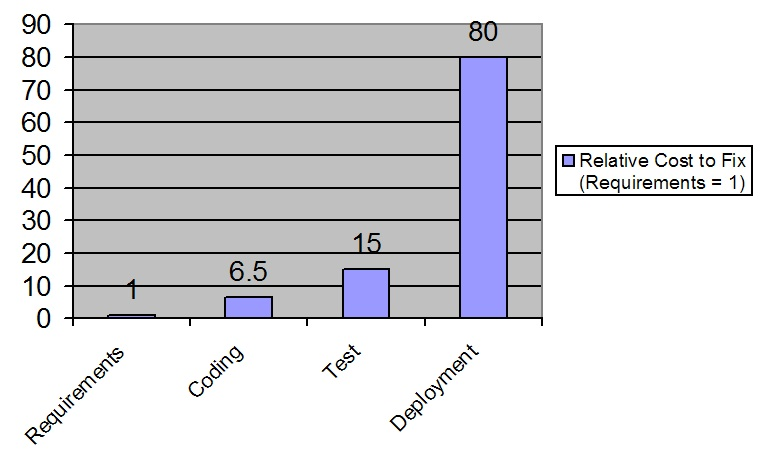
\includegraphics[width=0.9\textwidth]{requirement-error-cost.jpg}
    \caption[Costo della risoluzione di un errore avvenuto durante le attività di \textbf{analisi}]{Costo della risoluzione di un errore avvenuto durante le attività di \textbf{analisi} \footnotemark}
    \label{fig:req}
  \end{figure}
  {\footnotetext{Fonte: \href{https://www.stickyminds.com/article/what-cost-requirement-error}{https://www.stickyminds.com}}}

Nel mio caso, gli errori di comprensione sono stati risolti durante le attività di \textbf{analisi} stesse grazie alla volontà di tutte le parti di massimizzare il risultato in termini qualitativi e quantitativi, dato il vincolo di durata della mia esperienza lavorativa. \\
Altra competenza che ho acquisito nel corso delle attività di \textit{stage} è la gestione del tempo:
\begin{itemize}
    \item \textbf{Tempo dedicato ad attività produttive}: è importante identificare gli obiettivi principali per un periodo di tempo sufficiente ampio da consentire un avanzamento tangibile (ma non troppo ampio, per evitare di inserire un numero di obiettivi non realistico) e, a partire da questi obiettivi, pianificare i compiti e le attività per il periodo in analisi;
            la pianificazione dei compiti è ciò che consente di delineare una strategia di partenza e deve comprendere (per ogni compito) un periodo di tempo durante il quale il compito può essere in ritardo senza far tardare l'intero progetto di cui fa parte (\textit{slack time});
    \item \textbf{Tempo dedicato ad attività extra-lavorative}: una serie di circostanze personali mi ha permesso di sperimentare esattamente metà delle attività lavorative vivendo da solo, dovendo provvedere ai miei bisogni primari: questa esperienza mi ha fatto capire l'importanza della pianificazione anche nelle attività quotidiane, perseguendo la ripetibilità (e quindi instaurando una \textit{routine}) nelle attività che lo consentono,
            lasciando spazio e dando priorità quando possibile ad attività ricreative e sociali.
\end{itemize}

\section{Competenze curricolari e lavorative}
% In questa sezione discuterò della differenza tra le competenze acquisite ed erogate dal corso di studi e le competenze necessarie per lo svolgimento delle attività di tirocinio.
La distanza tra le competenze richieste all'inizio delle attività lavorative e quelle erogate dal corso di studi è minore di quanto avrei immaginato all'inizio dell'esperienza: 
\begin{itemize}
    \item \textbf{Gestione di progetto}: per quanto riguarda la gestione di progetto, affrontata durante i progetti didattici sviluppati per i corsi "Programmazione a Oggetti", "Tecnologie \textit{Web}" e "Ingegneria del \textit{Software}", 
            ho potuto constatare di aver colto gli elementi fondamentali per la buona riuscita di un progetto, specialmente se svolto in solitaria a livello di attività di sviluppo (come nel caso del tirocinio);
    \item \textbf{Ricerca di strumenti e tecnologie}: ho compreso durante gli studi che questa operazione è di grande impatto in un progetto e richiede abbastanza tempo e meticolosità per ottenere, in cambio, un prodotto che soddisfi determinate esigenze; proiettando questo ragionamento in un
            contesto lavorativo, una scelta errata può causare una perdita (economica e di tempo) ingente;
    \item \textbf{Comunicazione}: durante i progetti didattici ho avuto modo di capire l'importanza di una comunicazione chiara e celere con i colleghi e gli \glslink{stakeholder}{\textit{stakeholders}}, come evidenziato dalla figura \hyperref[fig:req]{4.1};
    \item \textbf{Conoscenza di strumenti moderni}: durante gli anni di studio ho potuto notare l'utilizzo di tecnologie consolidate per la spiegazione di concetti teorici e pratici quali il linguaggio \textit{C++} e l'insieme delle tecnologie alla base del \textit{web} (\hyperref[subsubsec:html]{\textit{HTML}}, \hyperref[subsubsec:css]{\textit{CSS}} e \textit{JavaScript});
            a mio parere, si sarebbe potuto dedicare del tempo per l'introduzione a tecnologie ormai anch'esse consolidate nel panorama dello sviluppo \textit{software} quali i \textit{framework} di sviluppo \textit{web} \textit{Angular} e \textit{React} ed i linguaggi di programmazione \textit{Kotlin} (per lo sviluppo di applicazioni \textit{Android}), \textit{Scala} e \textit{C\#}.
\end{itemize}